\item[(a)]
\section{Block Diagram of the LTI System}

\subsection*{Problem Statement}
Sketch the block diagram of the LTI system corresponding to the given difference equation:
\[ y[n] = x[n] - \frac{1}{15} y[n-1] + \frac{2}{5} y[n-2] \]

\subsection*{Theoretical Background}
A block diagram for an LTI (Linear Time-Invariant) system visually represents the flow of signals and the operations applied to them. The difference equation can be transformed into a block diagram using delay elements \( z^{-1} \), multipliers, and adders.

\subsection*{Mathematical Derivation}
The given difference equation is:
\[ y[n] = x[n] - \frac{1}{15} y[n-1] + \frac{2}{5} y[n-2] \]

This can be expressed in terms of block diagram components:
\begin{itemize}
    \item \( x[n] \) is the input signal.
    \item \( y[n] \) is the output signal.
    \item \( y[n-1] \) and \( y[n-2] \) are delayed versions of the output signal.
    \item Multipliers \( -\frac{1}{15} \) and \( \frac{2}{5} \) scale the delayed outputs.
    \item An adder combines the scaled delayed outputs with the input signal to produce the output.
\end{itemize}

\subsection*{Block Diagram}
The block diagram representation is as follows:

\begin{figure}[h]
    \centering
    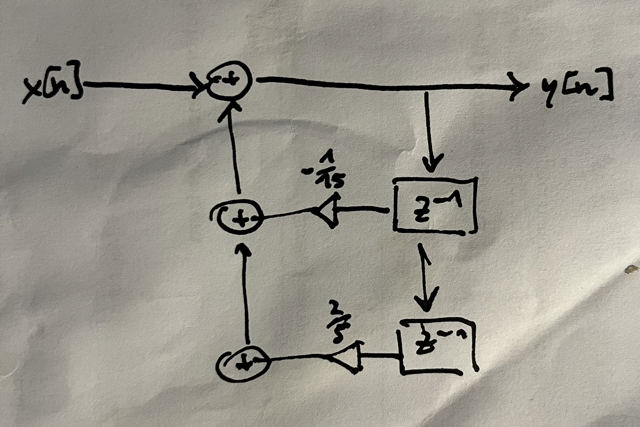
\includegraphics[width=0.8\textwidth]{fig/ex2_a_block_diagram.png}
    \caption{Block Diagram of the LTI System}
    \label{fig:ex2_a_block_diagram}
\end{figure}

\subsection*{Conclusion}
The block diagram illustrates the flow of the input signal \( x[n] \), the delayed outputs \( y[n-1] \) and \( y[n-2] \), and their scaled versions being combined to form the output signal \( y[n] \).
